% Framework figure for PSSA-VLA v2c (as actually implemented).
% Compile with:   pdflatex framework.tex
\documentclass[tikz,border=10pt]{standalone}
\usepackage{tikz}
\usepackage{xcolor}
\usetikzlibrary{positioning,arrows.meta,shapes,fit,calc,backgrounds}

\definecolor{cVis}{RGB}{56,103,214}
\definecolor{cLang}{RGB}{36,128,68}
\definecolor{cPSE}{RGB}{210,90,40}
\definecolor{cAct}{RGB}{120,60,160}
\definecolor{cCRED}{RGB}{200,40,80}
\definecolor{cFrozen}{RGB}{160,160,160}

\begin{document}
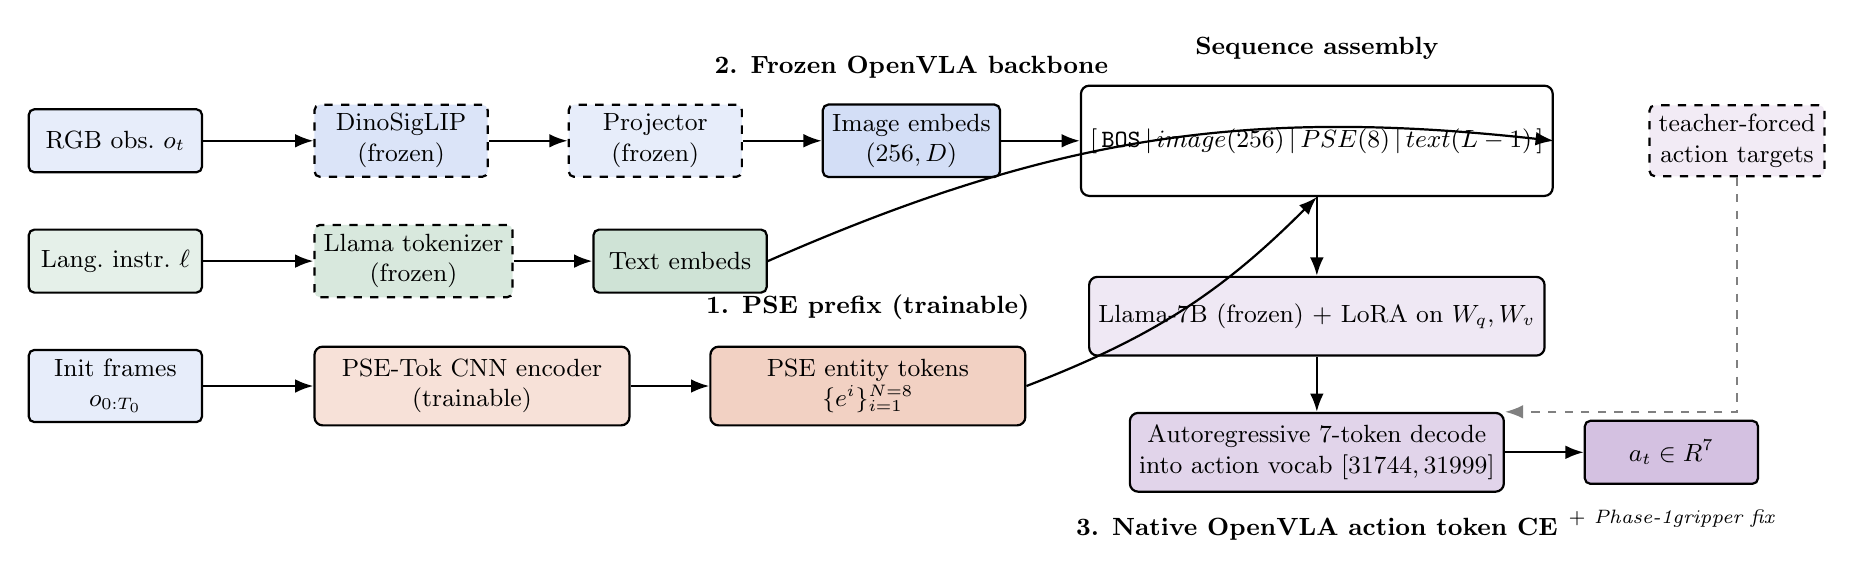
\begin{tikzpicture}[
    node distance=7mm and 10mm,
    every node/.style={font=\small},
    box/.style={draw,rounded corners=2pt,thick,minimum width=22mm,
                minimum height=8mm,align=center,fill=white},
    bigbox/.style={draw,rounded corners=3pt,thick,minimum width=40mm,
                   minimum height=10mm,align=center,fill=white},
    frozenbox/.style={draw,rounded corners=2pt,thick,minimum width=22mm,
                      minimum height=8mm,align=center,fill=cFrozen!15,
                      dashed},
    arrow/.style={-Latex,thick},
    dashedarrow/.style={-Latex,thick,dashed},
]

% --- Inputs ---
\node[box,fill=cVis!12]   (rgb)   at (0,0)        {RGB obs.\ $o_t$};
\node[box,fill=cLang!12,below=of rgb] (lang) {Lang.\ instr.\ $\ell$};
\node[box,fill=cVis!12,below=of lang] (rgbinit) {Init frames\\$o_{0:T_0}$};

% --- PSE encoder ---
\node[bigbox,fill=cPSE!18,right=14mm of rgbinit] (pse_enc) {PSE-Tok CNN encoder\\(trainable)};
\node[bigbox,fill=cPSE!28,right=of pse_enc] (pse_tok) {PSE entity tokens\\$\{e^i\}_{i=1}^{N=8}$};

% --- Image + text path (frozen OpenVLA backbone) ---
\node[frozenbox,fill=cVis!18,right=14mm of rgb] (dinosiglip) {DinoSigLIP\\(frozen)};
\node[frozenbox,fill=cVis!12,right=of dinosiglip] (proj) {Projector\\(frozen)};
\node[box,fill=cVis!22,right=of proj] (img_emb) {Image embeds\\$(256, D)$};

\node[frozenbox,fill=cLang!18,right=14mm of lang] (tok) {Llama tokenizer\\(frozen)};
\node[box,fill=cLang!22,right=of tok] (text_emb) {Text embeds};

% --- Sequence assembly ---
\node[bigbox,fill=white,thick,right=10mm of img_emb,minimum width=52mm,
      minimum height=14mm] (seq) {%
      $[\,\texttt{BOS}\,|\,\text{image}(256)\,|\,\text{PSE}(8)\,|\,\text{text}(L-1)\,]$};

% --- Llama + LoRA on q/v ---
\node[bigbox,fill=cAct!12,below=10mm of seq,minimum width=52mm] (llama) {%
    Llama-7B (frozen) $+$ LoRA on $W_q, W_v$};

% --- Action token decode ---
\node[bigbox,fill=cAct!22,below=of llama] (act_decode) {%
    Autoregressive 7-token decode\\into action vocab $[31744,31999]$};
\node[box,fill=cAct!32,right=of act_decode] (act) {$a_t \in \mathbb{R}^7$};

% --- Action target during training (teacher forcing) ---
\node[box,fill=cAct!10,right=of seq.east,xshift=2mm,dashed] (target) {%
    teacher-forced\\action targets};

% Edges
\draw[arrow] (rgb) -- (dinosiglip);
\draw[arrow] (dinosiglip) -- (proj);
\draw[arrow] (proj) -- (img_emb);
\draw[arrow] (lang) -- (tok);
\draw[arrow] (tok) -- (text_emb);
\draw[arrow] (rgbinit) -- (pse_enc);
\draw[arrow] (pse_enc) -- (pse_tok);

\draw[arrow] (img_emb) -- (seq);
\draw[arrow] (pse_tok.east) to[bend right=12] (seq.south);
\draw[arrow] (text_emb.east) to[bend left=15] (seq.east);

\draw[arrow] (seq) -- (llama);
\draw[arrow] (llama) -- (act_decode);
\draw[arrow] (act_decode) -- (act);

% Training-only path
\draw[dashedarrow,gray] (target.south) |- (act_decode.north east);

% Phase-1 eval gripper fix annotation
\node[font=\scriptsize\itshape,below=2mm of act] {$+$ Phase-1\\gripper fix};

% Titles
\node[font=\small\bfseries,above=2mm of seq] {Sequence assembly};
\node[font=\small\bfseries,above=2mm of pse_tok] {1. PSE prefix (trainable)};
\node[font=\small\bfseries,above=2mm of img_emb] {2. Frozen OpenVLA backbone};
\node[font=\small\bfseries,below=2mm of act_decode] {3. Native OpenVLA action token CE};

\end{tikzpicture}
\end{document}
